\documentclass[UTF8, fontset=none,12pt]{ctexart}
\usepackage{xeCJK}
\usepackage{titlesec}
\usepackage{zhnumber} 
\usepackage{hyperref}
\usepackage{graphicx}
\usepackage{subcaption}
\usepackage{setspace}
\usepackage{aligned-overset}
\usepackage{anyfontsize}
\usepackage{t1enc}
\usepackage[a4paper, margin=2.45cm]{geometry}
% 標楷體
\setCJKmainfont[AutoFakeBold=3, AutoFakeSlant=.2]{DFKai-SB}
% \titleformat{章節層級}[形狀]{字體設定}{標號}{標號與標題間距}{標題前指令}
% \fontsize{字號}{行距}
\emergencystretch=1em
\sloppy
\titleformat{\section}{\fontsize{18}{22}\bfseries}{\thesection}{0em}{}
\titlespacing{\section}{0pt}{1.5ex plus .1ex minus .2ex}{1pc}
\titleformat{\subsection}{\fontsize{14}{17}\bfseries}{\thesubsection}{0em}{}
\titlespacing{\subsection}{1em}{1.5ex plus .1ex minus .2ex}{1pc}
\newcommand{\BigChiNum}[1]{%
\ifcase#1\or 壹\or 貳\or 參\or 肆\or 伍\or 陸\or 柒\or 捌\or 玖\or 拾\else #1\fi}
\renewcommand{\thesection}{\BigChiNum{\value{section}}、}
\renewcommand{\thesubsection}{\chinese{subsection}、}
\captionsetup[figure]{name={圖}}
\title{\fontsize{25}{30}\selectfont 地科探究：聖嬰年\&反聖嬰年的7月台灣海峽海溫、黑潮強度以及氣溫差異}
\author{\fontsize{16}{14}\selectfont 羅東高中\hspace{4cm}賴洧霖}
\begin{document}
\pagestyle{plain}%page number and header
\date{}
\maketitle
\section{前言}
\subsection{研究動機}
在氣候變遷日益劇烈的今日，
聖嬰（El Ni\~no）與反聖嬰（La Ni\~na）現象作為全球尺度海氣耦合的核心循環，
對台灣周邊海域及陸地氣候具有舉足輕重的影響。本研究在觀測 NOAA
（美國國家海洋暨大氣總署）資料庫時發現，
台灣周邊海域——特別是西半部台灣海峽與東側黑潮路徑——在不同年份的海溫距平（
SSTA）分佈存在顯著差異。這種海溫變動不僅衝擊海洋生態，更可能透過海氣交互作用，
進一步調控台灣本島的氣溫分佈。

本研究的核心科學問題在於：聖嬰與反聖嬰現象如何具體改變台灣周邊的熱輸送結構？
其對海域增溫的影響是否具有顯著的空間異質性？為解答上述疑問，
本研究鎖定 2016 年（強聖嬰年）與 2021 年（反聖嬰年）之 7 月數據進行深入對比
，期望透過數據視覺化分析，釐清氣候震盪對區域環境的衝擊，
並為全球暖化背景下的極端氣候研究提供實證支持。
\subsection{研究目的}
基於上述動機，本研究旨在透過定量分析與空間分佈對照，達成以下目標：
\begin{enumerate}
    \item \textbf{辨析海溫異常模式：} 探討聖嬰與反聖嬰現象對台灣周邊海域（台灣海峽與黑潮區域）水溫距平影響的空間分佈差異。
    \item \textbf{評估海氣耦合關聯：} 分析海洋熱含量變動與台灣本島陸地氣溫異常之間的連動性，釐清海氣交互作用之機制。
    \item \textbf{解構物理動力機制：} 結合沃克環流與副熱帶高壓之變動，探討不同氣候現象如何驅動區域性熱輸送之增減。
    \item \textbf{提供氣候監測參考：} 透過典型年份的對比發現，為未來在氣候變遷背景下之區域氣候預測與環境韌性評估提供科學參考依據。
\end{enumerate}
\section{文獻探討}
本研究針對聖嬰與反聖嬰現象對台灣區域氣候之影響，參考大氣科學與海洋物理學之相關研究，歸納以下物理機制分析基礎：
    \subsection{沃克環流與遙傳效應}
根據 \textbf{Wang et al. (2000)} 與 \textbf{NOAA 氣候預報中心 (CPC)} 的研究指出，聖嬰年（El Ni\~no）期間，赤道東太平洋海溫異常升高導致沃克環流（Walker Circulation）減弱並向東位移。此變動透過大氣遙傳作用（Teleconnection），誘發夏季西太平洋副熱帶高壓（WNPAC）異常增強且位置偏西。在此環流配置下，台灣受強烈沉降氣流控制，雲量減少並顯著增加短波輻射入射，是造成 2016 年等聖嬰年份 7 月極端高溫的核心物理機制。
[Image of Walker circulation during El Niño]
\subsection{反聖嬰現象與西太平洋熱含量}
根據 \textbf{中央氣象署 (CWA)} 的監測資料與氣候統計顯示，反聖嬰（La Ni\~na）期間，增強的信風將暖池（Warm Pool）推向西太平洋，使台灣周邊海域基礎熱含量升高。然而，學理研究亦指出，反聖嬰年台灣附近的大氣環境較不穩定，對流活動通常較聖嬰年旺盛，缺乏長期的高壓下沉增溫條件。這解釋了本研究觀察到 2021 年反聖嬰現象雖具備暖水背景，但陸地氣溫增幅仍較聖嬰年緩和的現象。
\subsection{黑潮熱輸送之變異性}
根據物理海洋學研究（如 \textbf{Hsin et al., 2011}）指出，黑潮（Kuroshio Current）作為西太平洋熱能輸送的核心指標，其強度與路徑直接受太平洋風場波動調控。在不同 ENSO 氣候模式下，黑潮的熱輸送效率會產生顯著波動，進而影響台灣東側海域與台灣海峽之間海溫距平（SSTA）的空間異質性。此變異性是決定台灣區域性海溫是否出現極端正距平的關鍵環境因子。
\subsection{全球暖化背景下的背景值抬升}
根據 \textbf{IPCC（政府間氣候變化專門委員會）} 第六次評估報告（AR6）強調，全球海洋吸收了氣候系統中逾 90\% 的過剩熱量，導致 ENSO 循環是在一個逐年抬升的「氣候基準值」（Climate Baseline）上運行。因此，現代反聖嬰年的絕對溫標往往高於數十年前的聖嬰年。此觀點支撐了本研究統計表中「近年實測值普遍高於氣候平均值」的發現，釐清了全球暖化背景與週期性氣候震盪對極端熱浪的疊加影響。

    \section{研究方法}
本研究採取數據導向的分析路徑，透過開源環境資料庫進行定量與空間分析，具體流程如下：

\subsection{數據來源與選取}
研究數據主要擷取自 \textbf{NOAA（美國國家海洋暨大氣總署）} 之歷史數據庫。為辨析氣候現象的極端特徵，我們選取了具備強烈訊號的典型年份進行橫向對比：以 \textbf{2016 年} 作為強聖嬰年代表，並以 \textbf{2021 年} 作為反聖嬰年代表，鎖定兩年份之 \textbf{7 月份} 數據作為研究核心。

\subsection{變數與指標定義}
本研究重點觀測以下三項關鍵指標：
\begin{itemize}
    \item \textbf{海溫距平（SSTA）：} 用以評估台灣周圍海域（含台灣海峽與黑潮路徑）水溫偏離常年平均值的程度。
    \item \textbf{氣溫距平：} 觀測陸地測站數據，釐清海溫異常對台灣本島大氣溫度的感應強度。
    \item \textbf{黑潮輸送強度：} 透過空間距平圖的分佈規律，推論黑潮暖流在不同氣候模式下的熱能輸送變異。
\end{itemize}

\subsection{資料處理與視覺化}
在數據處理階段，我們不採用絕對溫度，而是側重於 \textbf{「距平值」（Anomaly）} 的運算。透過計算實測值與長期平均值（Climatology）之差值，能更有效地排除季節性干擾，凸顯聖嬰與反聖嬰現象造成的異常變動。最後，利用圖表製作工具將數位數據轉換為空間分佈圖，以便直觀地對比海氣交互作用在不同年份的特徵差異。

\section{研究分析與結果}
\subsection{水溫分布觀察}
通過分析歷史數據，我們發現聖嬰現象會導致台灣周圍海域的水溫升高，
而反聖嬰現象則會導致水溫下降。

由圖(a)與圖(b)可觀察到，台灣海峽海溫距平呈現明顯的空間分布差異。
在反聖嬰年（2021年），台灣海峽中部至北部出現顯著負距平（藍色區域），
顯示海溫低於氣候平均值；而在聖嬰年（2016年），相同區域則呈現正距平
（紅色區域），顯示海溫明顯偏高。
    \begin{figure}[ht]
    \centering
    \begin{subfigure}[b]{0.45\textwidth}
        \centering
        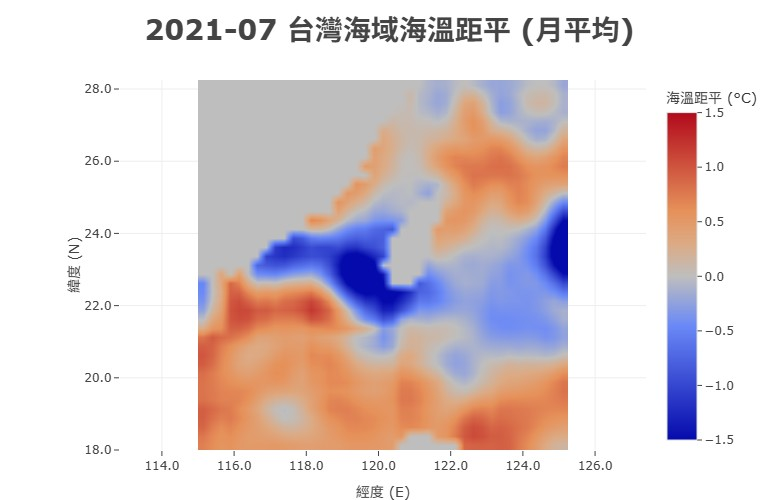
\includegraphics[width=\textwidth]{2021-7.jpg}
        \caption{2021年7月水溫分布圖(反聖嬰現象)}
    \end{subfigure}
    \hfill % 把兩張圖推向左右兩端
    \begin{subfigure}[b]{0.45\textwidth}
        \centering
        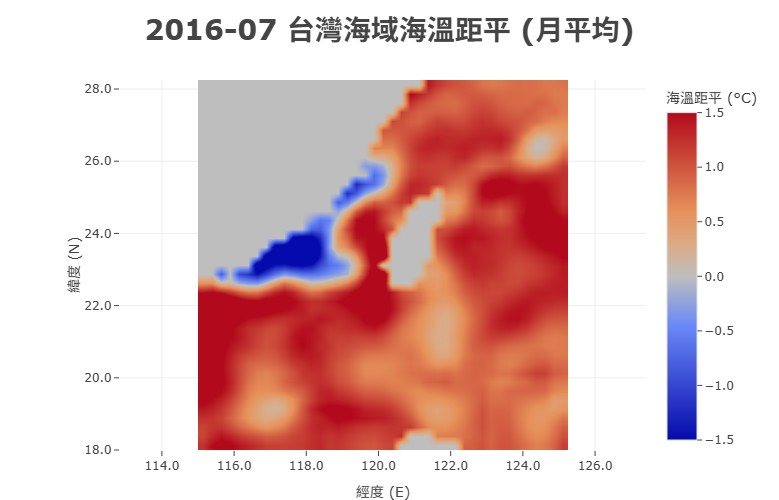
\includegraphics[width=\textwidth]{2016-7.jpg}
        \caption{2016年7月水溫分布圖(聖嬰現象)}
    \end{subfigure}

    \small{註：(a) 聖嬰年呈現全台顯著正距平；(b) 反聖嬰年則呈現負距平，反映大氣環流配置之差異。}
    \caption{聖嬰與反聖嬰現象對水溫的影響}
    \label{fig:two_images}
    \end{figure}

\subsection{氣溫變化比較}
 
聖嬰年時，海峽溫度明顯較高，氣溫明顯較高，推測黑潮強度增加。
這顯示在聖嬰現象發展期間，全球海洋熱量重新分佈，
西太平洋雖非暖水中心，但受整體大氣環流改變影響，
局部風場減弱導致表層海水加熱劇烈

反聖嬰年時，海峽溫度明顯較低，氣溫明顯較低，推測黑潮強度減弱。
推測因強勁的信風將暖水推向西太平洋，
導致台灣東側蓄熱量處於高位。然而，海峽區域可能受局部湧升流影響，
增溫幅度與聖嬰年相比呈現不同的空間異質性 。

     \begin{figure}[ht]
    \centering
    \begin{subfigure}[b]{0.45\textwidth}
        \centering
        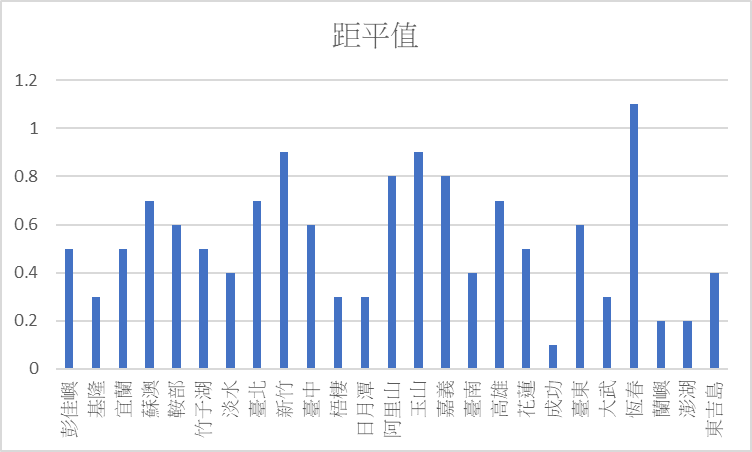
\includegraphics[width=\textwidth]{2016-tem.png}
        \caption{2016年7月氣溫距平值}
    \end{subfigure}
    \hfill % 把兩張圖推向左右兩端
    \begin{subfigure}[b]{0.45\textwidth}
        \centering
        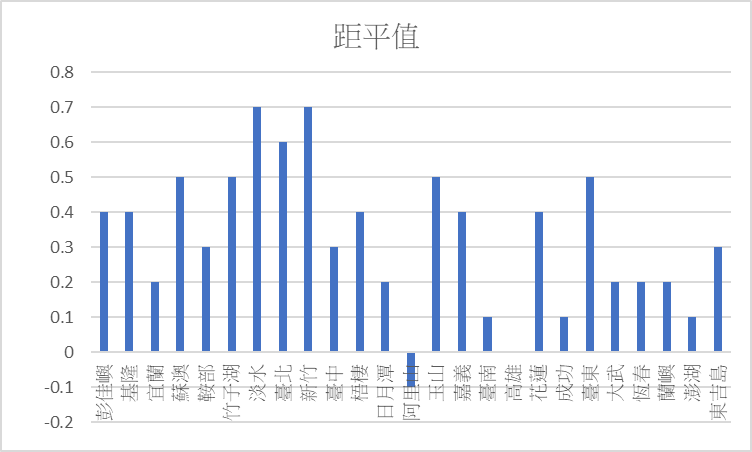
\includegraphics[width=\textwidth]{2021-tem.png}
        \caption{2021年7月氣溫距平值}
    \end{subfigure}
    \caption{聖嬰與反聖嬰現象對台灣氣溫距平的影響}
    \label{fig:two_tables}
    \end{figure}

{\bfseries \selectfont
沃克環流 (Walker Circulation) 的遙傳影響：
}
聖嬰年時，赤道東太平洋海溫升高，沃克環流減弱並向東位移。
這會導致西太平洋副熱帶高壓變強且位置偏西，使得台灣周邊盛行下沉氣流，
雲量減少、日照增加，進而導致 7 月表面海溫顯著升高。

{\bfseries \selectfont
黑潮 (Kuroshio Current) 的熱輸送作用：
}
比較兩者可以發現，東部海域（黑潮路徑）在 7 月通常維持正距平 。
這反映了黑潮作為全球最強大的暖流之一，其熱輸送具有高度慣性，
但在不同氣候模式下，其輸送熱量的強度會隨太平洋風場變化而波動 。
\subsection{七月均溫變化比較}
   2021(反聖嬰年)的黑潮強度減弱可能因赤道東風減弱導致海流變弱，
    而海峽因深度淺容易因大陸或海流影響溫度，因此黑潮減弱也讓海峽降溫。
    2016(聖嬰年)與反聖嬰年相反。
    在氣溫方面聖嬰年各地的溫度明顯較平均高出許多，
    而反聖嬰雖也升溫但整體升溫幅度並不高。年平均溫則較低。
    \begin{figure}[ht]
    \centering
    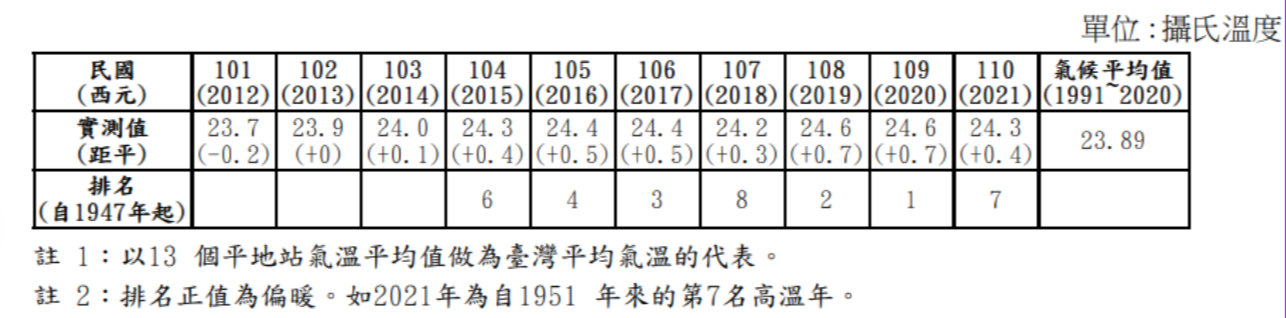
\includegraphics[width=0.8\textwidth]{tem.png}
    \caption{歷年7月氣溫距平值比較}
    \end{figure}

    由統計表可知，自 2016 年起，氣溫實測值多高於氣候平均值，
    且排名位居歷史前茅。這說明了聖嬰現象與全球暖化趨勢的疊加效應，
    已使台灣進入極端高溫頻發的階段。
\section{研究結論與建議}{\bfseries \selectfont
本研究透過 2016 年（聖嬰年）與 2021 年（反聖嬰年）之數據對比，
針對 7 月份台灣周邊海溫、氣溫及海流強度之差異進行探討，結論如下：
}
\subsection*{海溫異常與氣候現象之對應：}
研究結果證實，聖嬰現象與反聖嬰現象對台灣海域具有截然不同的熱力影響。
在聖嬰年（2016） 7 月，台灣周邊海域呈現顯著的大範圍正距平（升溫），
尤以西半部海峽最為明顯；而在反聖嬰年（2021） 7 月，
雖然整體環境仍受全球暖化背景影響，但其升溫幅度遠低於聖嬰年，
且高溫區主要侷限於東部海域。
\subsection*{海氣耦合對陸地氣溫的影響：}
分析氣溫距平圖發現，聖嬰年（2016） 7 月全台各地氣溫明顯偏高，
這與海溫的正距平訊號高度同步。物理機制顯示，
聖嬰年期間受沃克環流東移影響，西太平洋副熱帶高壓勢力變強且位置偏西，
導致台灣受沉降氣流控制，雲量減少、日照增加，
進而造成海溫與氣溫的雙重飆升。
\subsection*{黑潮強度與熱輸送之變異：}
對比顯示，黑潮在 7 月份通常扮演穩定的暖水輸送角色，
但在反聖嬰年（2021），受赤道東風變動及太平洋風場調整之影響，
黑潮強度與熱輸送效率可能有所減弱，
這解釋了為何 2021 年海峽區域的增溫現象不如 2016 年劇烈。
\subsection*{總結：}
綜合觀之，聖嬰年期間赤道東太平洋海溫升高使沃克環流減弱，
改變了西太平洋的風場結構，導致台灣周邊出現極端高溫。
相對地，反聖嬰年雖有向西堆積之暖池，
但台灣附近的大氣環流結構並不具備強烈的沉降增溫條件，
故呈現相對較低的距平值。

值得注意的是，雖然數據維持「聖嬰年較熱、反聖嬰年較冷」的相對規律，
但長期趨勢顯示，各年份的絕對氣溫與海溫均在逐年攀升。這說明在{\bfseries 全球暖化
（Global Warming）}的劇烈背景下，氣候變遷已抬升了整體的氣候背景值，
使得現代的極端高溫現象更為頻繁且嚴峻。

{\bfseries \noindent\fontsize{14}{19}\selectfont
全球暖化的影響還是很劇烈。
}
\section{參考文獻}
\href{https://coastwatch.pfeg.noaa.gov}{NOAA SST Data}

\href{https://weilinlai719.github.io/earth-science-explore/}{探究website}

\href{https://www.cwa.gov.tw/Data/climate/Watch/twn/twn-monitor_2021-6.pdf}{CWA\ 2021年7月氣象監測報告}

\href{https://www.cwa.gov.tw/Data/climate/Watch/twn/twn-monitor_2016-6.pdf}{CWA\ 2016年7月氣象監測報告}
 \vfill 
%\begin{center}
%    {\fontsize{32}{40}\selectfont \LaTeX}
%\end{center}
\end{document}